% Sección para integrar con % Sección para integrar con % Sección para integrar con % Sección para integrar con \input{lamport.tex} desde docs/.
% Requiere amsmath, booktabs, graphicx, caption, pdflscape, hyperref y biblatex.
\section{Verificación del reloj de Lamport}
\label{sec:lamport}

\subsection{Procedimiento y resultados de sockets}
Se analizaron los tres archivos \texttt{eventos\_sockets\_nodo-*.csv}
de la carpeta \texttt{data/}, correspondientes a los nodos A, B y C
en la corrida de sockets del 18 de noviembre de 2026.

El programa \texttt{analysis/}\allowbreak\texttt{verificar\_lamport.py} empareja los eventos.
Se usa el campo \texttt{id\_mensaje} y se comprueba que las
contrapartes coincidan. Para las actualizaciones locales se conserva el
orden de las filas de cada nodo y se parte de un reloj igual a cero.

Antes de un envío, el valor esperado es $L_{\mathrm{nuevo}}=L_{\mathrm{local}}+1$.
Al recibir un mensaje, debe cumplirse
$L_{\mathrm{nuevo}}=\max(L_{\mathrm{local}},L_{\mathrm{enviado}})+1$.
También se comprueba que
$L_{\text{recepción}}>L_{\text{envío}}$ para cada mensaje.
Estas reglas siguen el tratamiento de relojes lógicos y orden causal
de van Steen y Tanenbaum \cite{vansteen2023distributed}.
La comprobación se ejecuta desde la raíz del repositorio:

\begin{quote}\small\ttfamily
python analysis/verificar\_lamport.py\par
\normalfont\small con el argumento \texttt{"data/eventos\_sockets\_*.csv"}.
\end{quote}

\begin{table}[htbp]
\centering
\caption{Resultados obtenidos con los registros reales de sockets.}
\label{tab:lamport-resultados}
\begin{tabular}{lr}
\toprule
\textbf{Comprobación} & \textbf{Resultado} \\
\midrule
Nodos registrados & 3 \\
Eventos registrados & 42 \\
Mensajes con envío y recepción emparejados & 21 \\
Mensajes con $L_{\text{recepción}}>L_{\text{envío}}$ & 21 de 21 \\
Eventos que cumplen la regla de actualización & 42 de 42 \\
\bottomrule
\end{tabular}
\end{table}

\subsection{Dos eventos concurrentes con el mismo reloj}
En esta corrida se encontró el par de la tabla~\ref{tab:lamport-concurrentes}.
El envío de \texttt{cf648d87} se dirige a nodo-C, mientras que la
recepción de \texttt{a5cbb3c7} corresponde a otro mensaje.
El verificador construye las relaciones de precedencia a partir del orden
local y de cada enlace envío--recepción. Al recorrerlas, no encuentra
un camino desde uno de estos eventos hasta el otro en ninguna dirección.

\begin{table}[htbp]
\centering
\caption{Ejemplo de concurrencia en los registros de sockets.}
\label{tab:lamport-concurrentes}
\small
\begin{tabular}{lllll}
\toprule
\textbf{Nodo} & \textbf{Evento} & \textbf{Mensaje} & \textbf{Reloj} & \textbf{Hora local} \\
\midrule
nodo-A & envio & \texttt{cf648d87} & 2 & 10:50:25.829969 \\
nodo-B & recepcion & \texttt{a5cbb3c7} & 2 & 10:50:25.474609 \\
\bottomrule
\end{tabular}
\end{table}

Ambos eventos tienen reloj 2. Esto muestra que los relojes de Lamport no
asignan un número único a cada evento. La propiedad de orden causal
establece que, si un evento precede causalmente a otro, su reloj es menor.
El recíproco no permite deducir causalidad: un valor menor tampoco
basta para afirmar que hubo influencia entre dos eventos.
Para este ejemplo, la concurrencia se contrasta con las relaciones de
los registros completos de la corrida. La diferencia entre las horas
físicas no establece por sí sola una relación causal
\cite{vansteen2023distributed}.

\begin{landscape}
\subsection{Evidencia de ejecución}
La figura~\ref{fig:lamport-melanie} muestra la ejecución del verificador
con los registros de sockets del grupo. La captura incluye el usuario,
el nombre de la máquina, la fecha, la hora del sistema y la salida completa.
\begin{center}
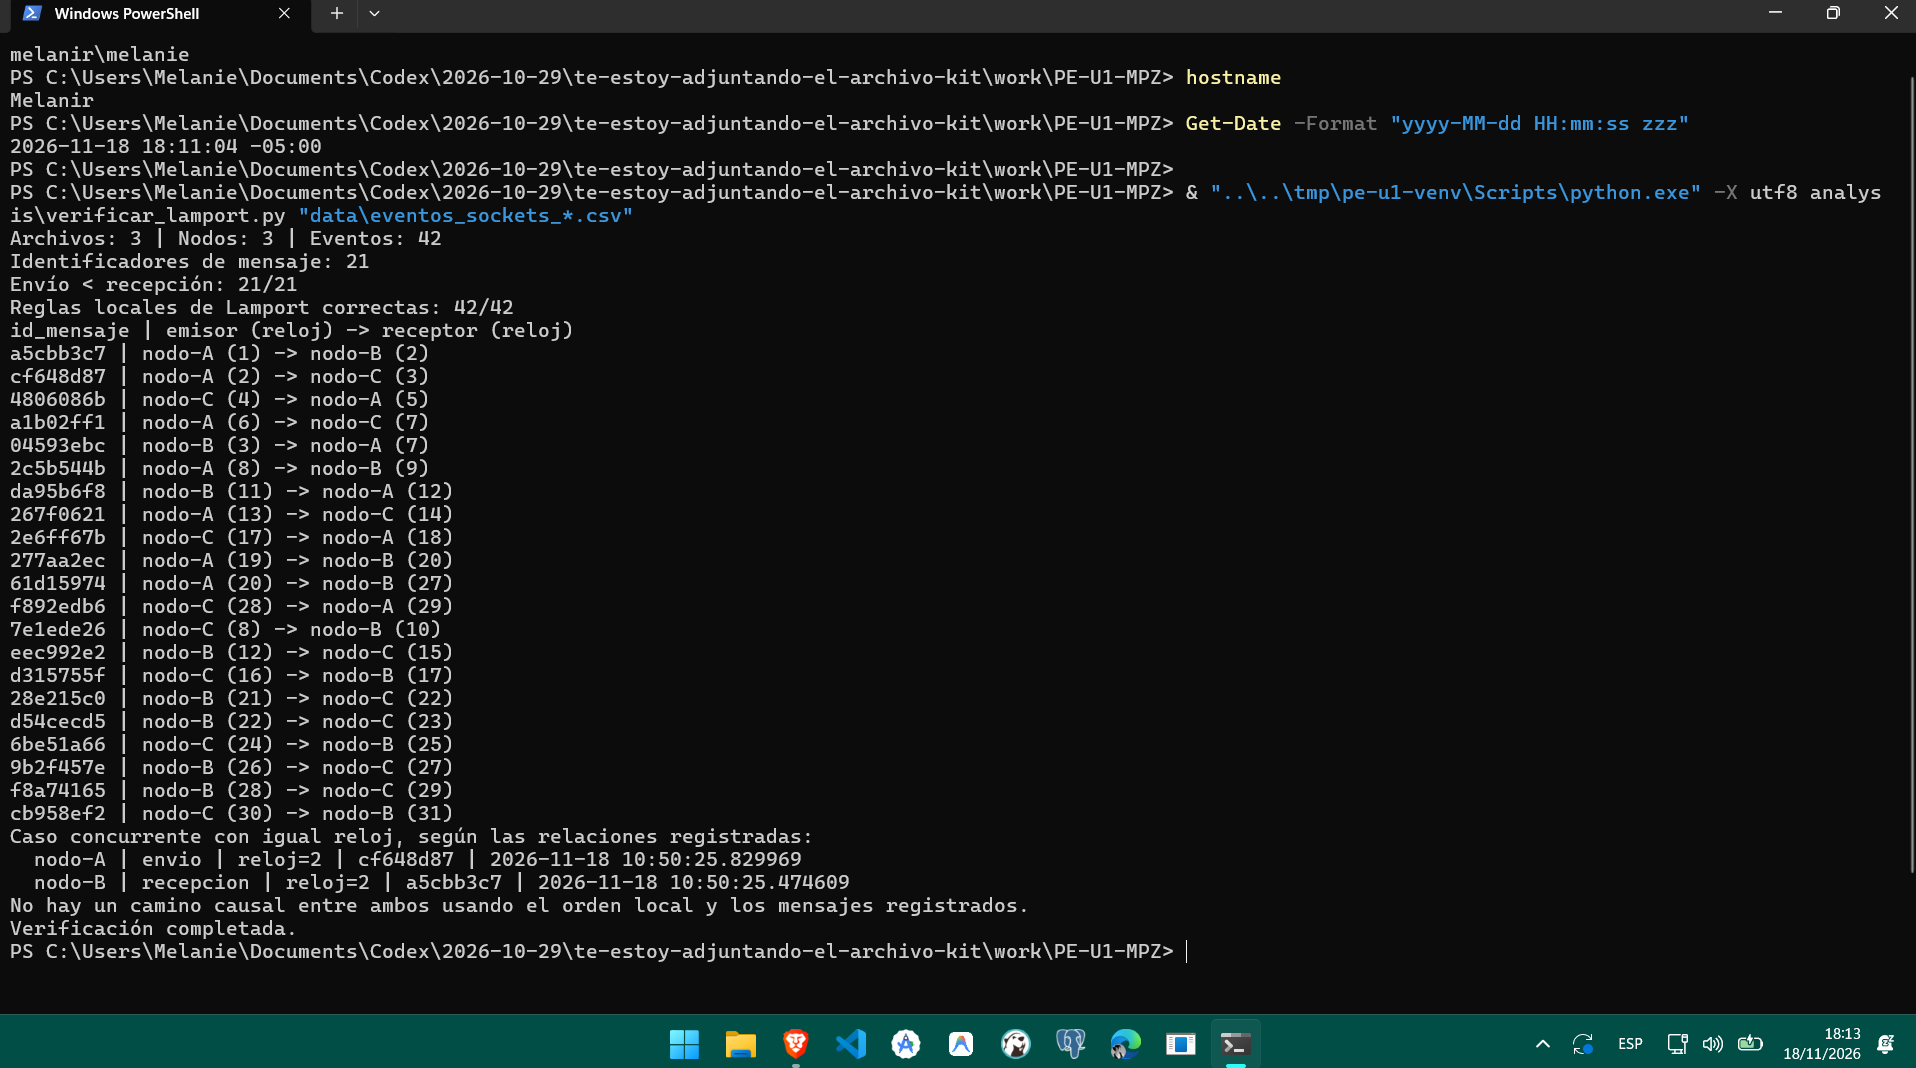
\includegraphics[width=\linewidth,height=0.72\textwidth,keepaspectratio]{../evidencias/melanie-verificacion-lamport.png}
\captionof{figure}{Ejecución del verificador de Lamport con los registros reales de sockets.}
\label{fig:lamport-melanie}
\end{center}
\end{landscape}
 desde docs/.
% Requiere amsmath, booktabs, graphicx, caption, pdflscape, hyperref y biblatex.
\section{Verificación del reloj de Lamport}
\label{sec:lamport}

\subsection{Procedimiento y resultados de sockets}
Se analizaron los tres archivos \texttt{eventos\_sockets\_nodo-*.csv}
de la carpeta \texttt{data/}, correspondientes a los nodos A, B y C
en la corrida de sockets del 18 de noviembre de 2026.

El programa \texttt{analysis/}\allowbreak\texttt{verificar\_lamport.py} empareja los eventos.
Se usa el campo \texttt{id\_mensaje} y se comprueba que las
contrapartes coincidan. Para las actualizaciones locales se conserva el
orden de las filas de cada nodo y se parte de un reloj igual a cero.

Antes de un envío, el valor esperado es $L_{\mathrm{nuevo}}=L_{\mathrm{local}}+1$.
Al recibir un mensaje, debe cumplirse
$L_{\mathrm{nuevo}}=\max(L_{\mathrm{local}},L_{\mathrm{enviado}})+1$.
También se comprueba que
$L_{\text{recepción}}>L_{\text{envío}}$ para cada mensaje.
Estas reglas siguen el tratamiento de relojes lógicos y orden causal
de van Steen y Tanenbaum \cite{vansteen2023distributed}.
La comprobación se ejecuta desde la raíz del repositorio:

\begin{quote}\small\ttfamily
python analysis/verificar\_lamport.py\par
\normalfont\small con el argumento \texttt{"data/eventos\_sockets\_*.csv"}.
\end{quote}

\begin{table}[htbp]
\centering
\caption{Resultados obtenidos con los registros reales de sockets.}
\label{tab:lamport-resultados}
\begin{tabular}{lr}
\toprule
\textbf{Comprobación} & \textbf{Resultado} \\
\midrule
Nodos registrados & 3 \\
Eventos registrados & 42 \\
Mensajes con envío y recepción emparejados & 21 \\
Mensajes con $L_{\text{recepción}}>L_{\text{envío}}$ & 21 de 21 \\
Eventos que cumplen la regla de actualización & 42 de 42 \\
\bottomrule
\end{tabular}
\end{table}

\subsection{Dos eventos concurrentes con el mismo reloj}
En esta corrida se encontró el par de la tabla~\ref{tab:lamport-concurrentes}.
El envío de \texttt{cf648d87} se dirige a nodo-C, mientras que la
recepción de \texttt{a5cbb3c7} corresponde a otro mensaje.
El verificador construye las relaciones de precedencia a partir del orden
local y de cada enlace envío--recepción. Al recorrerlas, no encuentra
un camino desde uno de estos eventos hasta el otro en ninguna dirección.

\begin{table}[htbp]
\centering
\caption{Ejemplo de concurrencia en los registros de sockets.}
\label{tab:lamport-concurrentes}
\small
\begin{tabular}{lllll}
\toprule
\textbf{Nodo} & \textbf{Evento} & \textbf{Mensaje} & \textbf{Reloj} & \textbf{Hora local} \\
\midrule
nodo-A & envio & \texttt{cf648d87} & 2 & 10:50:25.829969 \\
nodo-B & recepcion & \texttt{a5cbb3c7} & 2 & 10:50:25.474609 \\
\bottomrule
\end{tabular}
\end{table}

Ambos eventos tienen reloj 2. Esto muestra que los relojes de Lamport no
asignan un número único a cada evento. La propiedad de orden causal
establece que, si un evento precede causalmente a otro, su reloj es menor.
El recíproco no permite deducir causalidad: un valor menor tampoco
basta para afirmar que hubo influencia entre dos eventos.
Para este ejemplo, la concurrencia se contrasta con las relaciones de
los registros completos de la corrida. La diferencia entre las horas
físicas no establece por sí sola una relación causal
\cite{vansteen2023distributed}.

\begin{landscape}
\subsection{Evidencia de ejecución}
La figura~\ref{fig:lamport-melanie} muestra la ejecución del verificador
con los registros de sockets del grupo. La captura incluye el usuario,
el nombre de la máquina, la fecha, la hora del sistema y la salida completa.
\begin{center}
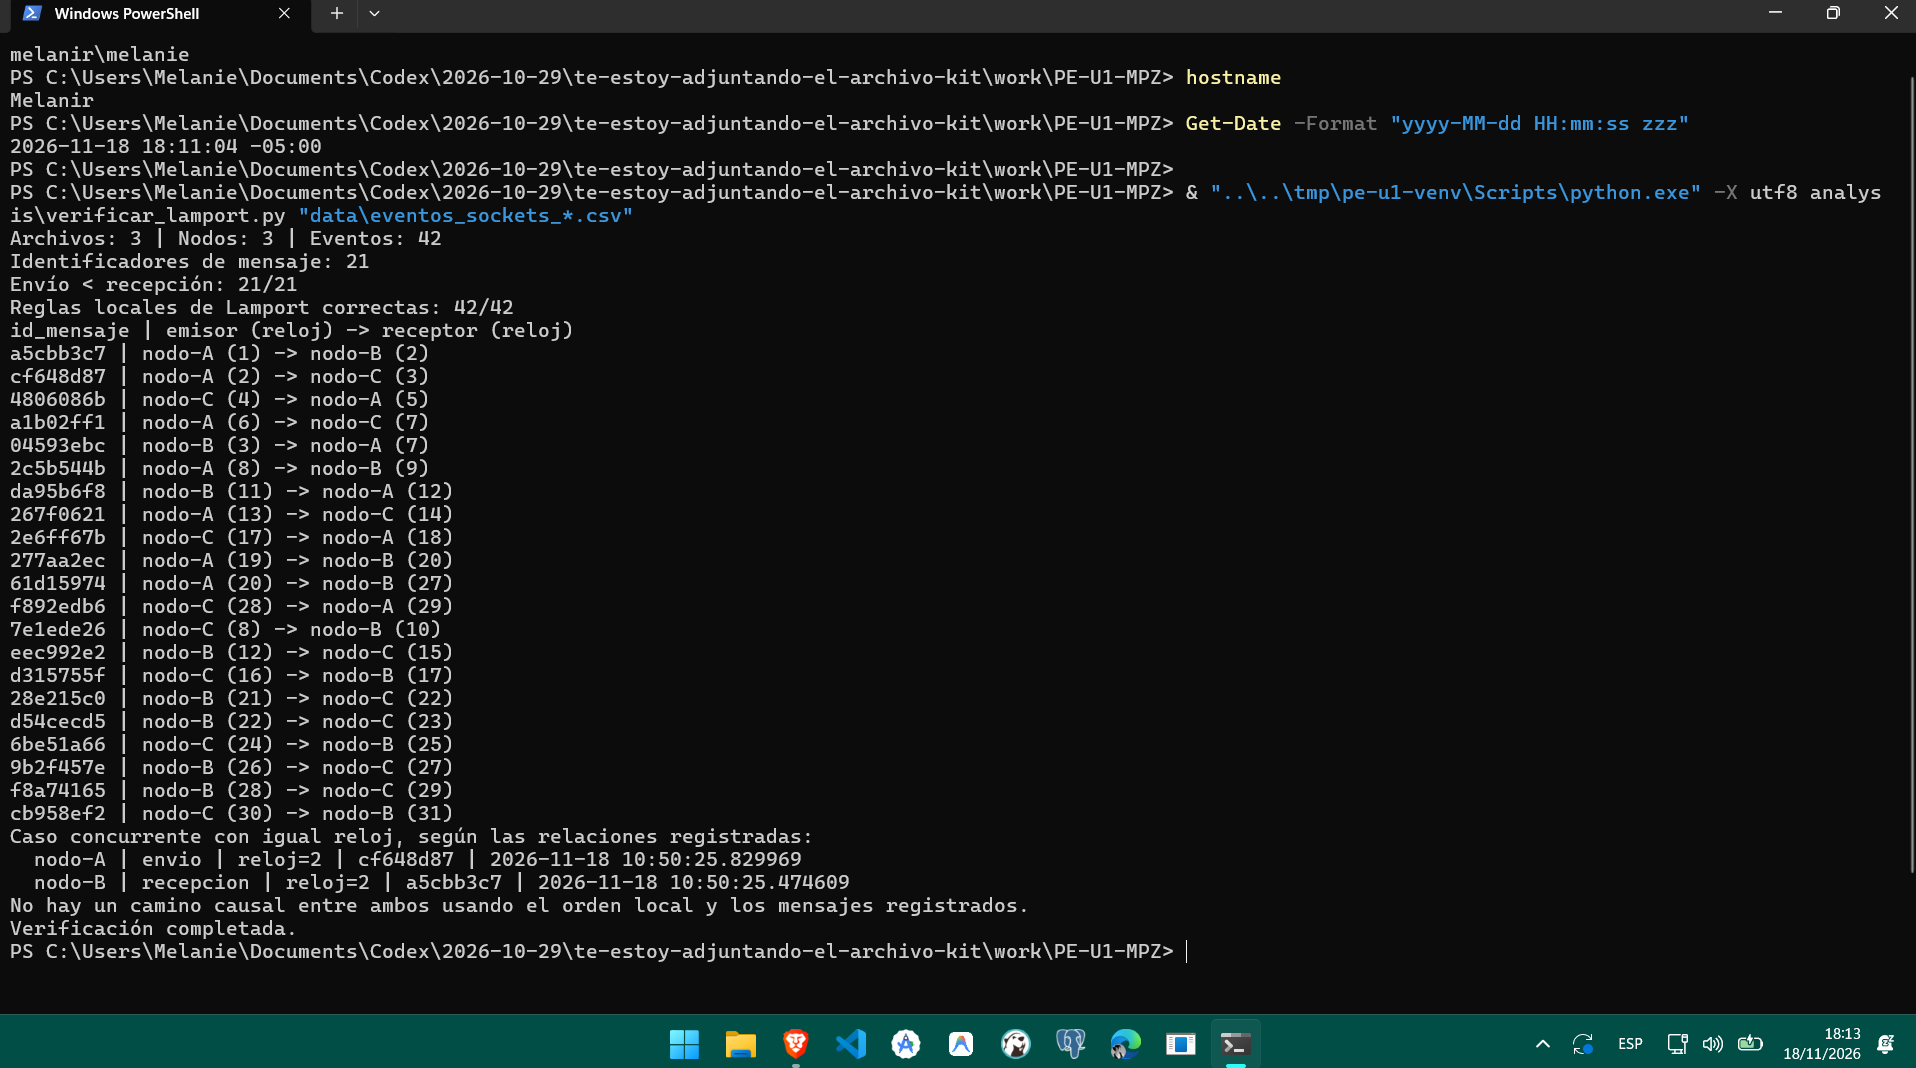
\includegraphics[width=\linewidth,height=0.72\textwidth,keepaspectratio]{../evidencias/melanie-verificacion-lamport.png}
\captionof{figure}{Ejecución del verificador de Lamport con los registros reales de sockets.}
\label{fig:lamport-melanie}
\end{center}
\end{landscape}
 desde docs/.
% Requiere amsmath, booktabs, graphicx, caption, pdflscape, hyperref y biblatex.
\section{Verificación del reloj de Lamport}
\label{sec:lamport}

\subsection{Procedimiento y resultados de sockets}
Se analizaron los tres archivos \texttt{eventos\_sockets\_nodo-*.csv}
de la carpeta \texttt{data/}, correspondientes a los nodos A, B y C
en la corrida de sockets del 18 de noviembre de 2026.

El programa \texttt{analysis/}\allowbreak\texttt{verificar\_lamport.py} empareja los eventos.
Se usa el campo \texttt{id\_mensaje} y se comprueba que las
contrapartes coincidan. Para las actualizaciones locales se conserva el
orden de las filas de cada nodo y se parte de un reloj igual a cero.

Antes de un envío, el valor esperado es $L_{\mathrm{nuevo}}=L_{\mathrm{local}}+1$.
Al recibir un mensaje, debe cumplirse
$L_{\mathrm{nuevo}}=\max(L_{\mathrm{local}},L_{\mathrm{enviado}})+1$.
También se comprueba que
$L_{\text{recepción}}>L_{\text{envío}}$ para cada mensaje.
Estas reglas siguen el tratamiento de relojes lógicos y orden causal
de van Steen y Tanenbaum \cite{vansteen2023distributed}.
La comprobación se ejecuta desde la raíz del repositorio:

\begin{quote}\small\ttfamily
python analysis/verificar\_lamport.py\par
\normalfont\small con el argumento \texttt{"data/eventos\_sockets\_*.csv"}.
\end{quote}

\begin{table}[htbp]
\centering
\caption{Resultados obtenidos con los registros reales de sockets.}
\label{tab:lamport-resultados}
\begin{tabular}{lr}
\toprule
\textbf{Comprobación} & \textbf{Resultado} \\
\midrule
Nodos registrados & 3 \\
Eventos registrados & 42 \\
Mensajes con envío y recepción emparejados & 21 \\
Mensajes con $L_{\text{recepción}}>L_{\text{envío}}$ & 21 de 21 \\
Eventos que cumplen la regla de actualización & 42 de 42 \\
\bottomrule
\end{tabular}
\end{table}

\subsection{Dos eventos concurrentes con el mismo reloj}
En esta corrida se encontró el par de la tabla~\ref{tab:lamport-concurrentes}.
El envío de \texttt{cf648d87} se dirige a nodo-C, mientras que la
recepción de \texttt{a5cbb3c7} corresponde a otro mensaje.
El verificador construye las relaciones de precedencia a partir del orden
local y de cada enlace envío--recepción. Al recorrerlas, no encuentra
un camino desde uno de estos eventos hasta el otro en ninguna dirección.

\begin{table}[htbp]
\centering
\caption{Ejemplo de concurrencia en los registros de sockets.}
\label{tab:lamport-concurrentes}
\small
\begin{tabular}{lllll}
\toprule
\textbf{Nodo} & \textbf{Evento} & \textbf{Mensaje} & \textbf{Reloj} & \textbf{Hora local} \\
\midrule
nodo-A & envio & \texttt{cf648d87} & 2 & 10:50:25.829969 \\
nodo-B & recepcion & \texttt{a5cbb3c7} & 2 & 10:50:25.474609 \\
\bottomrule
\end{tabular}
\end{table}

Ambos eventos tienen reloj 2. Esto muestra que los relojes de Lamport no
asignan un número único a cada evento. La propiedad de orden causal
establece que, si un evento precede causalmente a otro, su reloj es menor.
El recíproco no permite deducir causalidad: un valor menor tampoco
basta para afirmar que hubo influencia entre dos eventos.
Para este ejemplo, la concurrencia se contrasta con las relaciones de
los registros completos de la corrida. La diferencia entre las horas
físicas no establece por sí sola una relación causal
\cite{vansteen2023distributed}.

\begin{landscape}
\subsection{Evidencia de ejecución}
La figura~\ref{fig:lamport-melanie} muestra la ejecución del verificador
con los registros de sockets del grupo. La captura incluye el usuario,
el nombre de la máquina, la fecha, la hora del sistema y la salida completa.
\begin{center}
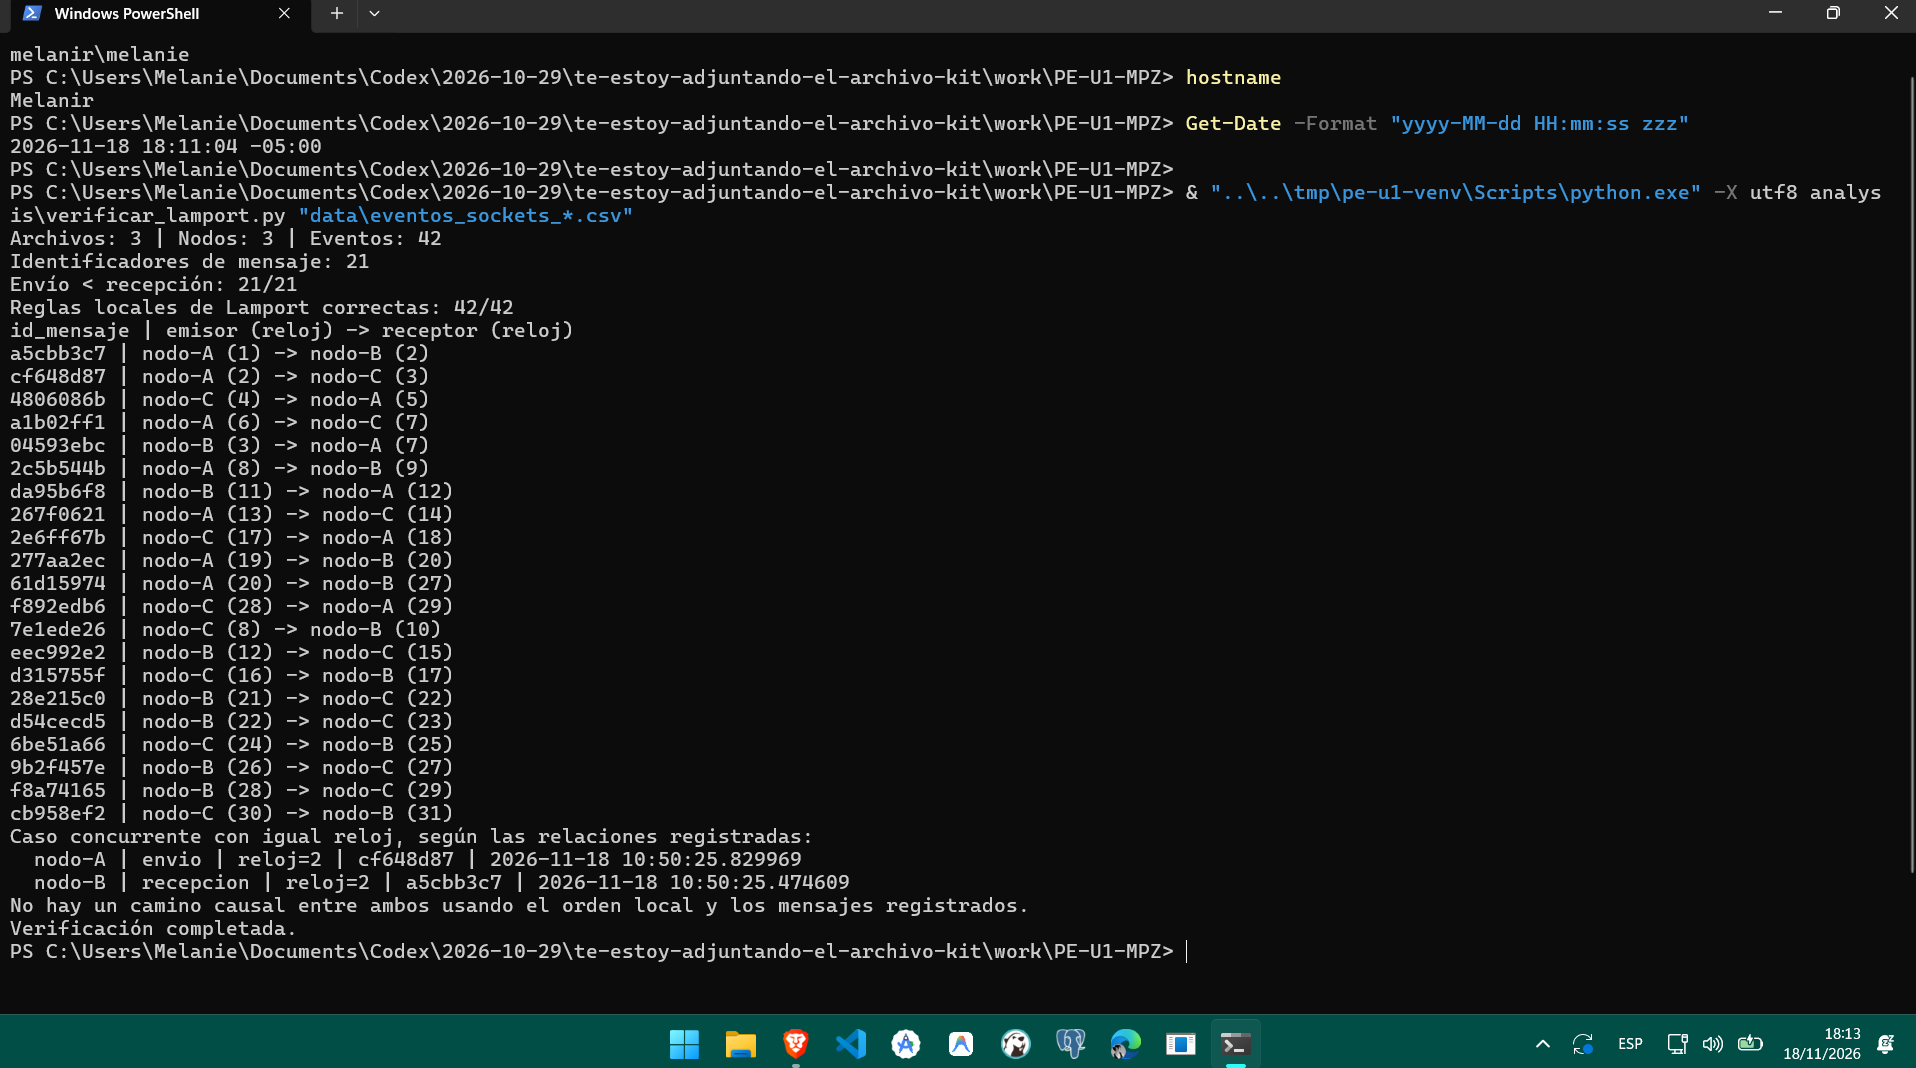
\includegraphics[width=\linewidth,height=0.72\textwidth,keepaspectratio]{../evidencias/melanie-verificacion-lamport.png}
\captionof{figure}{Ejecución del verificador de Lamport con los registros reales de sockets.}
\label{fig:lamport-melanie}
\end{center}
\end{landscape}
 desde docs/.
% Requiere amsmath, booktabs, graphicx, caption, pdflscape, hyperref y biblatex.
\section{Verificación del reloj de Lamport}
\label{sec:lamport}

\subsection{Procedimiento y resultados de sockets}
Se analizaron los tres archivos \texttt{eventos\_sockets\_nodo-*.csv}
de la carpeta \texttt{data/}, correspondientes a los nodos A, B y C
en la corrida de sockets del 18 de noviembre de 2026.

El programa \texttt{analysis/}\allowbreak\texttt{verificar\_lamport.py} empareja los eventos.
Se usa el campo \texttt{id\_mensaje} y se comprueba que las
contrapartes coincidan. Para las actualizaciones locales se conserva el
orden de las filas de cada nodo y se parte de un reloj igual a cero.

Antes de un envío, el valor esperado es $L_{\mathrm{nuevo}}=L_{\mathrm{local}}+1$.
Al recibir un mensaje, debe cumplirse
$L_{\mathrm{nuevo}}=\max(L_{\mathrm{local}},L_{\mathrm{enviado}})+1$.
También se comprueba que
$L_{\text{recepción}}>L_{\text{envío}}$ para cada mensaje.
Estas reglas siguen el tratamiento de relojes lógicos y orden causal
de van Steen y Tanenbaum \cite{vansteen2023distributed}.
La comprobación se ejecuta desde la raíz del repositorio:

\begin{quote}\small\ttfamily
python analysis/verificar\_lamport.py\par
\normalfont\small con el argumento \texttt{"data/eventos\_sockets\_*.csv"}.
\end{quote}

\begin{table}[htbp]
\centering
\caption{Resultados obtenidos con los registros reales de sockets.}
\label{tab:lamport-resultados}
\begin{tabular}{lr}
\toprule
\textbf{Comprobación} & \textbf{Resultado} \\
\midrule
Nodos registrados & 3 \\
Eventos registrados & 42 \\
Mensajes con envío y recepción emparejados & 21 \\
Mensajes con $L_{\text{recepción}}>L_{\text{envío}}$ & 21 de 21 \\
Eventos que cumplen la regla de actualización & 42 de 42 \\
\bottomrule
\end{tabular}
\end{table}

\subsection{Dos eventos concurrentes con el mismo reloj}
En esta corrida se encontró el par de la tabla~\ref{tab:lamport-concurrentes}.
El envío de \texttt{cf648d87} se dirige a nodo-C, mientras que la
recepción de \texttt{a5cbb3c7} corresponde a otro mensaje.
El verificador construye las relaciones de precedencia a partir del orden
local y de cada enlace envío--recepción. Al recorrerlas, no encuentra
un camino desde uno de estos eventos hasta el otro en ninguna dirección.

\begin{table}[htbp]
\centering
\caption{Ejemplo de concurrencia en los registros de sockets.}
\label{tab:lamport-concurrentes}
\small
\begin{tabular}{lllll}
\toprule
\textbf{Nodo} & \textbf{Evento} & \textbf{Mensaje} & \textbf{Reloj} & \textbf{Hora local} \\
\midrule
nodo-A & envio & \texttt{cf648d87} & 2 & 10:50:25.829969 \\
nodo-B & recepcion & \texttt{a5cbb3c7} & 2 & 10:50:25.474609 \\
\bottomrule
\end{tabular}
\end{table}

Ambos eventos tienen reloj 2. Esto muestra que los relojes de Lamport no
asignan un número único a cada evento. La propiedad de orden causal
establece que, si un evento precede causalmente a otro, su reloj es menor.
El recíproco no permite deducir causalidad: un valor menor tampoco
basta para afirmar que hubo influencia entre dos eventos.
Para este ejemplo, la concurrencia se contrasta con las relaciones de
los registros completos de la corrida. La diferencia entre las horas
físicas no establece por sí sola una relación causal
\cite{vansteen2023distributed}.

\begin{landscape}
\subsection{Evidencia de ejecución}
La figura~\ref{fig:lamport-melanie} muestra la ejecución del verificador
con los registros de sockets del grupo. La captura incluye el usuario,
el nombre de la máquina, la fecha, la hora del sistema y la salida completa.
\begin{center}
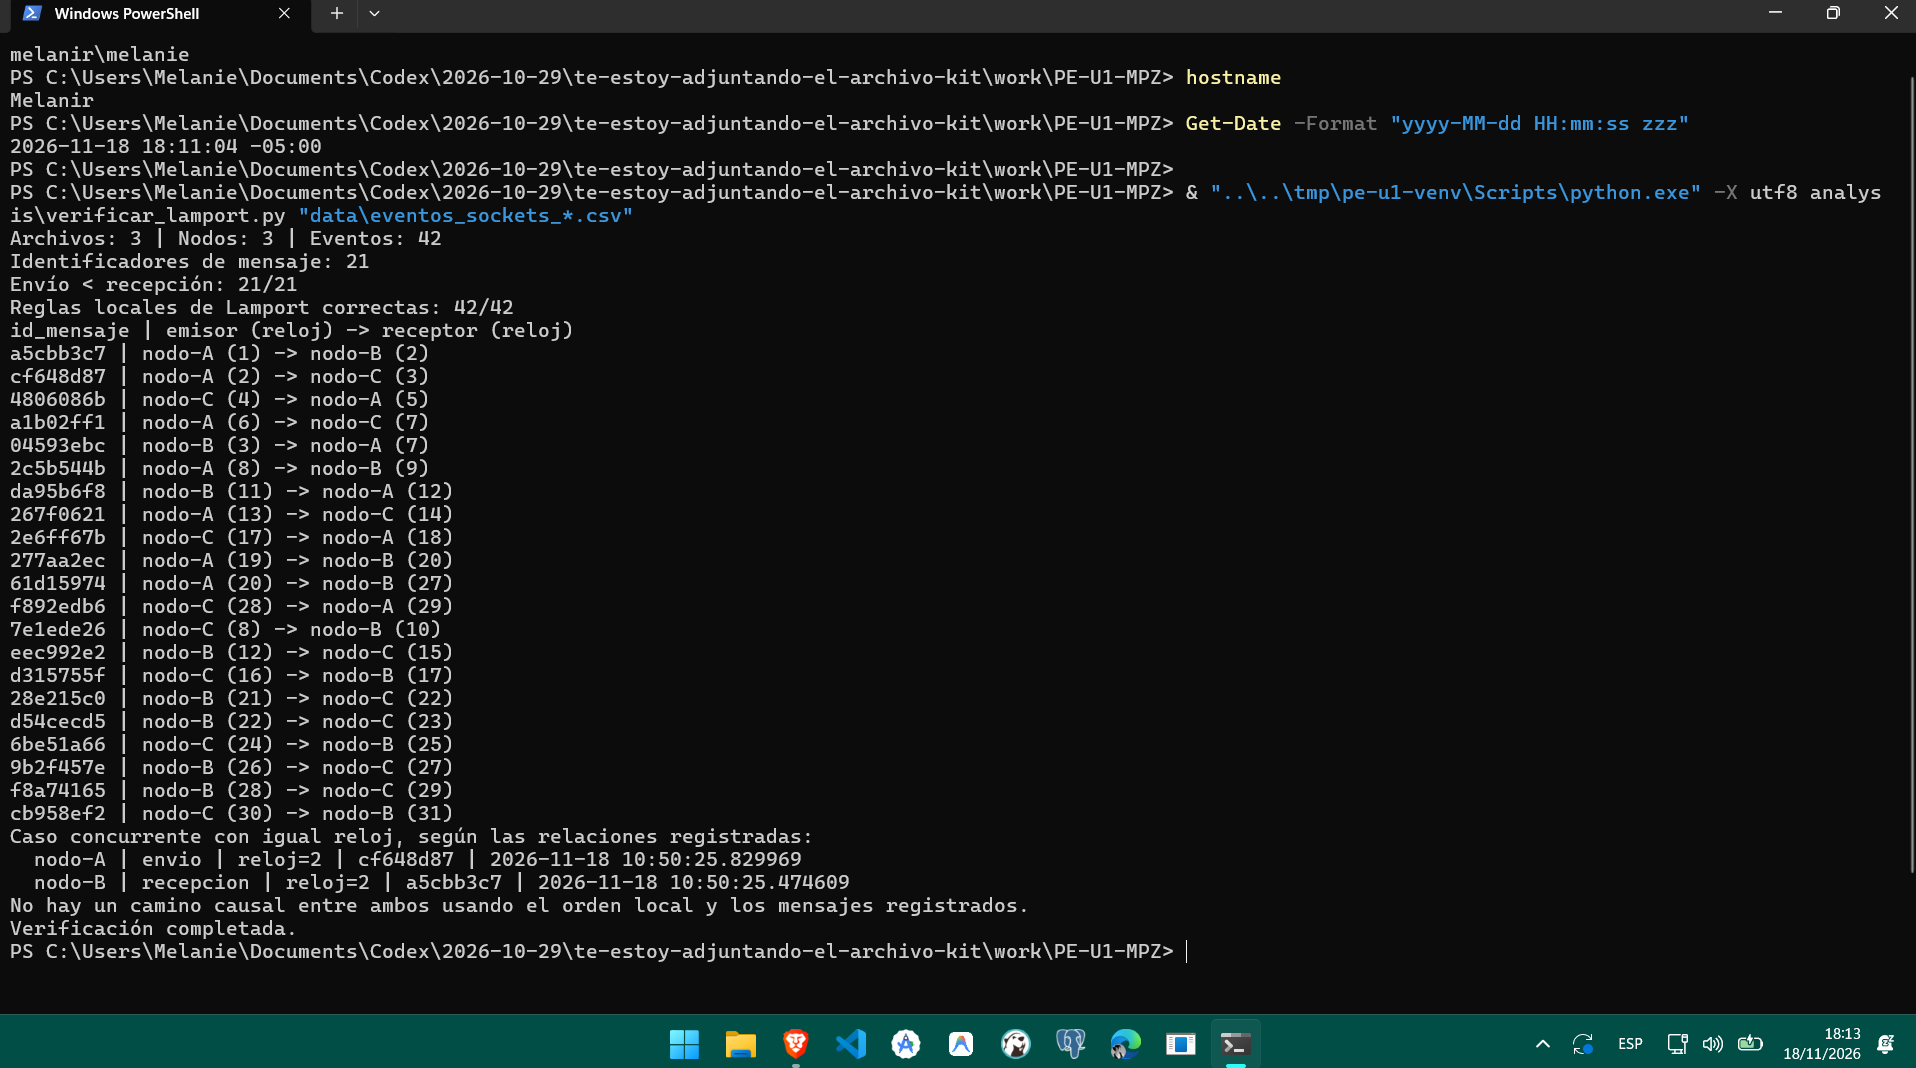
\includegraphics[width=\linewidth,height=0.72\textwidth,keepaspectratio]{../evidencias/melanie-verificacion-lamport.png}
\captionof{figure}{Ejecución del verificador de Lamport con los registros reales de sockets.}
\label{fig:lamport-melanie}
\end{center}
\end{landscape}
